% ============================================================================
% Práctica: instalación del framework V2X (VaN3Twin + SUMO + SUMO-GEO)
% Universidad de Cuenca — Redes Vehiculares y Heterogéneas (INGE-00104)
% Compilar: pdflatex -interaction=nonstopmode Practica_Instalacion_Framework.tex (x2)
% ============================================================================
\documentclass[11pt,a4paper]{article}

\usepackage[utf8]{inputenc}
\usepackage[T1]{fontenc}
\usepackage{lmodern}
\usepackage{amssymb}
\usepackage[margin=2.2cm]{geometry}
\usepackage{xcolor}
\usepackage{graphicx}
\usepackage{booktabs}
\usepackage{enumitem}
\usepackage{fancyhdr}
\usepackage{tikz}
\usetikzlibrary{positioning,arrows.meta,shapes.geometric}
\usepackage{listings}
\usepackage[most]{tcolorbox}
\usepackage{hyperref}

\definecolor{azul}{HTML}{002856}
\definecolor{rojo}{HTML}{A51008}
\definecolor{gris}{HTML}{58585B}
\definecolor{verde}{HTML}{1A7A4A}
\definecolor{fondocodigo}{HTML}{F5F5F5}

\hypersetup{colorlinks=true, linkcolor=azul, urlcolor=rojo, citecolor=azul}

\pagestyle{fancy}
\fancyhf{}
\fancyhead[L]{\small\color{azul}\textbf{Práctica · Instalación del framework V2X}}
\fancyhead[R]{\small\color{gris}Redes Vehiculares y Heterogéneas}
\fancyfoot[C]{\small\thepage}
\renewcommand{\headrulewidth}{0.6pt}

\lstdefinestyle{codigo}{
  backgroundcolor=\color{fondocodigo},
  basicstyle=\ttfamily\footnotesize,
  keywordstyle=\color{azul}\bfseries,
  commentstyle=\color{verde}\itshape,
  stringstyle=\color{rojo},
  numbers=none, breaklines=true, frame=single,
  rulecolor=\color{gris!40}, framesep=4pt,
  showstringspaces=false, tabsize=2, columns=fullflexible, keepspaces=true }
\lstset{style=codigo}

\newtcolorbox{terminalbox}[1][]{colback=azul!4, colframe=azul, fonttitle=\bfseries, breakable,
  title={TERMINAL #1}}
\newtcolorbox{encontenedor}[1][]{colback=rojo!4, colframe=rojo, fonttitle=\bfseries, breakable,
  title={DENTRO DEL CONTENEDOR \texttt{van3twin} #1}}
\newtcolorbox{ennavegador}[1][]{colback=verde!5, colframe=verde, fonttitle=\bfseries, breakable,
  title={EN EL NAVEGADOR #1}}
\newtcolorbox{notabox}[1][]{colback=gris!6, colframe=gris, fonttitle=\bfseries, breakable,
  title={Nota#1}}
\newtcolorbox{advertenciabox}{colback=rojo!6, colframe=rojo, fonttitle=\bfseries, breakable,
  title={Advertencia}}
\newtcolorbox{previobox}{colback=azul!6, colframe=azul, fonttitle=\bfseries, breakable,
  title={TRABAJO PREVIO --- traer HECHO a la clase}}
\newtcolorbox{checkbox}[1][]{colback=verde!6, colframe=verde, fonttitle=\bfseries, breakable,
  title={$\checkmark$ Verificación#1}}

\setlength{\parskip}{4pt}
\setlength{\parindent}{0pt}
\renewcommand{\contentsname}{Contenido}

% ============================================================================
\begin{document}

\begin{center}
  {\color{azul}\LARGE\bfseries Instalación del framework V2X}\\[4pt]
  {\color{gris}\large VaN3Twin (ns-3) + SUMO + visor 3D SUMO-GEO, con Docker, en Linux, Windows y macOS}\\[6pt]
  {\small Universidad de Cuenca --- Redes Vehiculares y Heterogéneas (INGE-00104)\\
  Prof.\ Pablo Barbecho --- 28 de agosto de 2026}
\end{center}

\vspace{2pt}\hrule\vspace{8pt}

\tableofcontents

% ============================================================================
\section{Objetivo}
% ============================================================================

Instalar y poner en marcha, en tu propio computador, el entorno completo de
simulación V2X del curso: el framework \textbf{VaN3Twin} (comunicaciones
vehiculares sobre ns-3), el simulador de movilidad \textbf{SUMO} y el visor
web 3D \textbf{SUMO-GEO}. Al terminar sabrás verificar cada componente por
separado y ejecutar una simulación integrada viéndola en vivo en el navegador
--- la base sobre la que trabajan las demás prácticas del curso.

% ============================================================================
\section{Marco teórico}
% ============================================================================

\subsection{Los componentes del framework}

\begin{itemize}[leftmargin=1.6em, itemsep=2pt]
  \item \textbf{SUMO} (\emph{Simulation of Urban MObility}): simulador
        microscópico de tráfico. Aporta la \emph{movilidad}: mapas, rutas y
        el movimiento de cada vehículo.
  \item \textbf{ns-3 + VaN3Twin}: ns-3 es el simulador de redes de referencia
        en investigación; VaN3Twin (evolución de ms-van3t, Politecnico di
        Torino) le añade la pila vehicular ETSI ITS-G5 completa (mensajes
        CAM/DENM/CPM reales en ASN.1) sobre 802.11p, LTE, C-V2X o NR-V2X.
  \item \textbf{TraCI} (\emph{Traffic Control Interface}): el puente. ns-3 se
        conecta a SUMO por un socket TCP y ambos avanzan sincronizados: SUMO
        mueve los vehículos, ns-3 simula sus comunicaciones.
  \item \textbf{SUMO-GEO}: visor web (backend Python FastAPI + frontend
        MapLibre/deck.gl) que se conecta a SUMO como \emph{segundo} cliente
        TraCI de solo lectura y dibuja la simulación en 3D sobre el mapa
        real, en el navegador. Incluye además un modo \emph{replay} que
        reproduce corridas grabadas (.pcap) con el intercambio de mensajes.
\end{itemize}

\begin{figure}[h!]
\centering
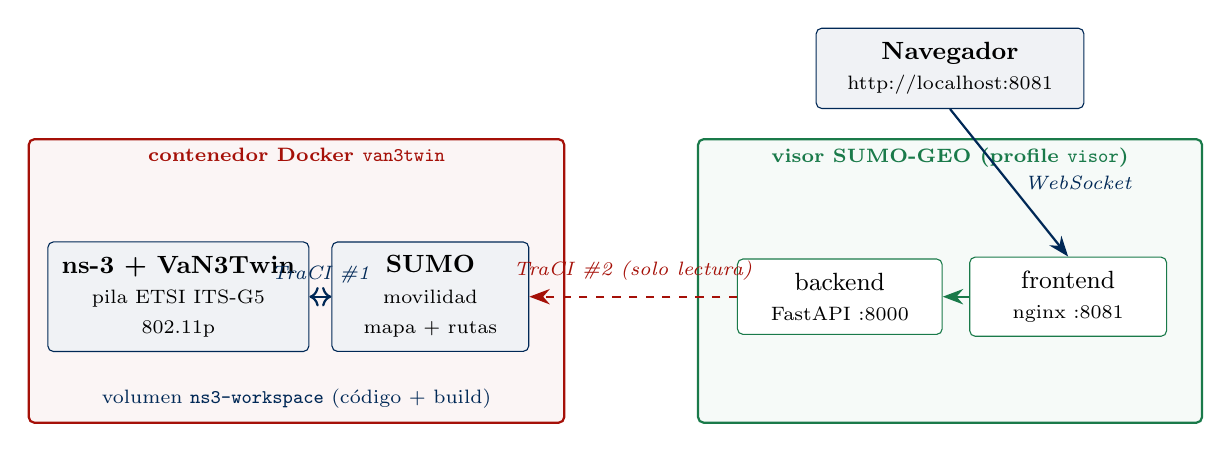
\begin{tikzpicture}[
  font=\small,
  caja/.style={draw, rounded corners=2pt, align=center, inner sep=5pt},
  flecha/.style={-{Stealth[length=2.6mm]}, thick},
  etiq/.style={font=\scriptsize\itshape, midway}
]
  \node[caja, draw=rojo, thick, fill=rojo!4, minimum width=6.8cm, minimum height=3.6cm] (van) at (-4.1,0) {};
  \node[anchor=north, font=\scriptsize\bfseries\color{rojo}] at (van.north) {contenedor Docker \texttt{van3twin}};
  \node[caja, draw=azul, fill=azul!6, minimum width=2.7cm] (ns3) at (-5.6,-0.2)
        {\textbf{ns-3 + VaN3Twin}\\\scriptsize pila ETSI ITS-G5\\\scriptsize 802.11p};
  \node[caja, draw=azul, fill=azul!6, minimum width=2.5cm] (sumo) at (-2.4,-0.2)
        {\textbf{SUMO}\\\scriptsize movilidad\\\scriptsize mapa + rutas};
  \draw[flecha, azul, <->] (ns3) -- (sumo) node[etiq, above=1pt] {TraCI \#1};
  \node[font=\scriptsize\color{azul}] at (-4.1,-1.5) {volumen \texttt{ns3-workspace} (código + build)};

  \node[caja, draw=verde, thick, fill=verde!4, minimum width=6.4cm, minimum height=3.6cm] (geo) at (4.2,0) {};
  \node[anchor=north, font=\scriptsize\bfseries\color{verde}] at (geo.north) {visor SUMO-GEO (profile \texttt{visor})};
  \node[caja, draw=verde, fill=white, minimum width=2.6cm] (backend) at (2.8,-0.2)
        {backend\\\scriptsize FastAPI :8000};
  \node[caja, draw=verde, fill=white, minimum width=2.5cm] (nginx) at (5.7,-0.2)
        {frontend\\\scriptsize nginx :8081};
  \draw[flecha, verde] (nginx) -- (backend);
  \draw[flecha, rojo, dashed, thick] (backend.west) -- (sumo.east)
        node[etiq, above=2pt] {TraCI \#2 (solo lectura)};
  \node[caja, draw=azul, fill=azul!6, minimum width=3.4cm] (br) at (4.2,2.7)
        {\textbf{Navegador}\\\scriptsize http://localhost:8081};
  \draw[flecha, azul, thick] (br.south) -- (nginx.north) node[etiq, right=2pt] {WebSocket};
\end{tikzpicture}
\caption{Arquitectura en ejecución: SUMO acepta dos clientes TraCI (ns-3
controla; el visor solo lee) y avanza en \emph{lockstep} con ambos.}
\label{fig:arq}
\end{figure}

\subsection{Los repositorios y qué papel juega cada uno}

Todo se despliega desde GitHub (figura~\ref{fig:repos}). Solo se clonan
\textbf{dos} repos --- el tercero (el código ns-3) lo clona Docker
\emph{dentro de la imagen} durante la construcción, lo que además evita un
problema serio de sistemas de ficheros (§\ref{sec:fs}).

\begin{center}
\small
\begin{tabular}{@{}lp{0.30\textwidth}p{0.38\textwidth}@{}}
\toprule
\textbf{Repo (github.com/Pbarbecho)} & \textbf{Contenido} & \textbf{¿Se clona a mano?} \\
\midrule
\texttt{van3twin-docker} & Dockerfile, \texttt{docker-compose.yml}, manuales y prácticas & \textbf{Sí} — punto de entrada \\
\texttt{SUMO\_GEO} & Visor web (backend + frontend) & \textbf{Sí} — junto al anterior \\
\texttt{VaN3TwinGEO} & Fork de VaN3Twin con los parches de la integración & \textbf{No} — lo clona el build de Docker dentro de la imagen \\
\bottomrule
\end{tabular}
\end{center}

\begin{figure}[h!]
\centering
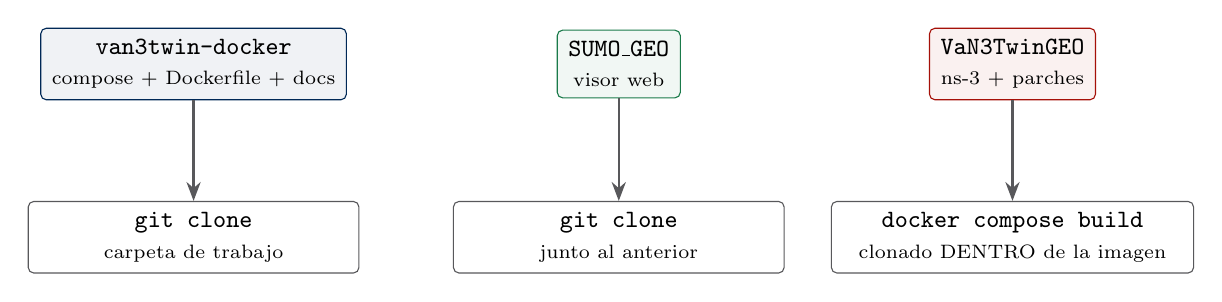
\begin{tikzpicture}[
  font=\small,
  caja/.style={draw, rounded corners=2pt, align=center, inner sep=4pt},
  flecha/.style={-{Stealth[length=2.4mm]}, thick, gris}
]
  \node[caja, draw=azul, fill=azul!6] (r1) at (0,2.2) {\texttt{van3twin-docker}\\\scriptsize compose + Dockerfile + docs};
  \node[caja, draw=verde, fill=verde!6] (r2) at (5.4,2.2) {\texttt{SUMO\_GEO}\\\scriptsize visor web};
  \node[caja, draw=rojo, fill=rojo!6] (r3) at (10.4,2.2) {\texttt{VaN3TwinGEO}\\\scriptsize ns-3 + parches};
  \node[caja, draw=gris, minimum width=4.2cm] (pc) at (0,0) {\texttt{git clone}\\\scriptsize carpeta de trabajo};
  \node[caja, draw=gris, minimum width=4.2cm] (pc2) at (5.4,0) {\texttt{git clone}\\\scriptsize junto al anterior};
  \node[caja, draw=gris, minimum width=4.6cm] (img) at (10.4,0) {\texttt{docker compose build}\\\scriptsize clonado DENTRO de la imagen};
  \draw[flecha] (r1) -- (pc);
  \draw[flecha] (r2) -- (pc2);
  \draw[flecha] (r3) -- (img);
\end{tikzpicture}
\caption{De GitHub a tu máquina: dos clones manuales; el código ns-3 viaja
dentro de la imagen Docker.}
\label{fig:repos}
\end{figure}

\subsection{¿Por qué Docker? Imagen, contenedor y volumen}

El entorno nativo de VaN3Twin exige Ubuntu, decenas de dependencias y horas
de compilación. Docker lo empaqueta: la \textbf{imagen} es una plantilla
inmutable (Ubuntu 22.04 + SUMO + gRPC + ns-3 \emph{ya compilado}); un
\textbf{contenedor} es una instancia en ejecución de esa imagen; un
\textbf{volumen} es un disco persistente gestionado por Docker --- aquí, el
volumen \texttt{ns3-workspace} guarda el árbol de código y sobrevive aunque
el contenedor se destruya. \textbf{Docker Compose} describe en un YAML los
servicios (contenedores), sus redes, puertos y volúmenes, y los orquesta con
un solo comando. Los \emph{profiles} permiten grupos opcionales: aquí el
visor solo arranca si se pide \texttt{-{}-profile visor}.

\subsection{\texttt{docker} vs.\ \texttt{docker compose}, y desde qué carpeta ejecutarlos}

Son dos niveles de la misma herramienta:

\begin{itemize}[leftmargin=1.6em, itemsep=2pt]
  \item \textbf{\texttt{docker} a secas} opera sobre objetos \emph{globales}
        del demonio (imágenes, contenedores, volúmenes, identificados por
        nombre). Sirve para acciones puntuales: \texttt{docker images},
        \texttt{docker ps}, \texttt{docker exec -it van3twin bash},
        \texttt{docker logs}. Como los nombres son globales,
        \textbf{funciona desde cualquier carpeta}.
  \item \textbf{\texttt{docker compose}} opera sobre un \emph{proyecto}:
        el conjunto de servicios, redes y volúmenes descrito en un
        \texttt{docker-compose.yml}. Por eso \textbf{debe ejecutarse en la
        carpeta donde está ese fichero} (o señalarlo con
        \texttt{-f ruta/al/compose.yml}). Si lo lanzas en otra carpeta,
        obtendrás \texttt{no configuration file provided: not found}; y si en
        esa otra carpeta hubiera \emph{otro} compose, estarías manejando
        \textbf{otro proyecto distinto} sin darte cuenta.
\end{itemize}

En este curso eso significa: los \texttt{docker compose ...} del stack se
lanzan desde \texttt{van3twin-docker/}; el del visor autónomo (nivel 3 de la
verificación), desde \texttt{SUMO\_GEO/}. Son dos proyectos independientes
--- con contenedores, redes y volúmenes propios --- que casualmente comparten
los puertos 8000/8081, y por eso no pueden estar arriba a la vez. Algo
parecido pasa con \texttt{docker build}: la ruta que le pasas (el
\emph{contexto}, p.\,ej.\ el ``\texttt{.}'' de \texttt{docker build -t x .})
define dónde busca el \texttt{Dockerfile} y qué ficheros puede copiar dentro
de la imagen; \texttt{docker compose build} hace esto solo, leyendo la ruta
del YAML.

\subsection{Los ficheros del proyecto: qué es cada uno y cuándo lo usamos}

\begin{center}
\small
\begin{tabular}{@{}p{0.34\textwidth}p{0.30\textwidth}p{0.28\textwidth}@{}}
\toprule
\textbf{Fichero} & \textbf{Qué es} & \textbf{Cuándo lo usamos} \\
\midrule
\texttt{van3twin-docker/Dockerfile} & Receta de la imagen \texttt{van3twin}: Ubuntu + SUMO + gRPC + clona el fork y compila ns-3, capa a capa & Solo indirectamente, vía \texttt{docker compose build} (trabajo previo); no se edita \\
\texttt{van3twin-docker/docker-compose.yml} & \textbf{El fichero central}: define los servicios \texttt{van3twin}, \texttt{backend} y \texttt{frontend} (profile \texttt{visor}), el volumen \texttt{ns3-workspace}, puertos y montajes & En cada \texttt{up / exec / logs / stop} del día a día \\
\texttt{van3twin-docker/.env} & Variables locales de TU máquina (p.\,ej.\ \texttt{SUMO\_GEO\_DIR}); compose lo lee solo & Solo si \texttt{SUMO\_GEO} no está junto a \texttt{van3twin-docker} \\
\texttt{SUMO\_GEO/docker-compose.yml} & Proyecto \emph{independiente}: el visor autónomo (modo \emph{managed}, escenarios de Cuenca) & Solo en el nivel 3 de verificación; después, \texttt{down} \\
\texttt{SUMO\_GEO/backend/Dockerfile.van3twin} & Receta de la imagen del backend en modo integrado (Python slim + traci 1.12, sin binario SUMO) & Indirectamente: la construye el \texttt{-{}-profile visor} del compose central \\
\texttt{SUMO\_GEO/backend/Dockerfile} & Receta del backend autónomo (incluye SUMO completo) & Indirectamente, solo en el nivel 3 \\
\texttt{SUMO\_GEO/frontend/} (html/js/css + \texttt{nginx.conf}) & El visor que ves en el navegador; nginx lo sirve \emph{montado}, sin construir imagen & Siempre que abres \texttt{localhost:8081}; los cambios se ven con recargar \\
\bottomrule
\end{tabular}
\end{center}

\subsection{El problema de las mayúsculas (léelo antes de clonar)}
\label{sec:fs}

El repo de ns-3/VaN3Twin contiene pares de ficheros que \textbf{solo difieren
en mayúsculas} (\texttt{ActionID.c}/\texttt{ActionId.c},
\texttt{BOOLEAN.h}/\texttt{boolean.h}\ldots). En Linux (ext4) son dos
ficheros distintos; en los sistemas de ficheros por defecto de
\textbf{Windows (NTFS)} y \textbf{macOS (APFS)}, que no distinguen
mayúsculas, uno \emph{machaca} al otro al clonar y el árbol queda corrupto
--- git incluso avisa (``paths have collided''). Por eso el diseño del
framework: \textbf{el código ns-3 nunca toca tu disco}; vive dentro de la
imagen y del volumen Docker (Linux, case-sensitive). Los dos repos que sí
clonas no tienen este problema.

\subsection{Repaso exprés de git}

\begin{center}
\small
\begin{tabular}{@{}ll@{}}
\toprule
\textbf{Comando} & \textbf{Qué hace} \\
\midrule
\texttt{git clone <url>} & Descarga un repositorio completo (código + historial) \\
\texttt{git status} & Estado: rama actual, ficheros modificados \\
\texttt{git log -{}-oneline -5} & Últimos 5 commits \\
\texttt{git pull} & Trae los cambios nuevos del remoto (actualizarse) \\
\texttt{git branch} / \texttt{git checkout <rama>} & Listar / cambiar de rama \\
\texttt{git diff} & Ver qué cambió respecto al último commit \\
\texttt{git add <f>} + \texttt{git commit -m "..."} & Registrar cambios propios \\
\texttt{git remote -v} & Ver a qué URL apunta el repo \\
\bottomrule
\end{tabular}
\end{center}

\subsection{Repaso exprés de Docker y Compose}

\begin{center}
\small
\begin{tabular}{@{}ll@{}}
\toprule
\textbf{Comando} & \textbf{Qué hace} \\
\midrule
\texttt{docker images} / \texttt{docker ps -a} & Imágenes locales / contenedores (todos) \\
\texttt{docker compose build} & Construye las imágenes del compose \\
\texttt{docker compose up -d} & Crea y arranca los servicios (en segundo plano) \\
\texttt{docker compose -{}-profile visor up -d} & Ídem incluyendo el grupo opcional \texttt{visor} \\
\texttt{docker compose ps} & Estado de los servicios del proyecto \\
\texttt{docker compose exec van3twin bash} & Shell dentro del contenedor \\
\texttt{docker compose logs <servicio>} & Logs de un servicio (depuración) \\
\texttt{docker compose stop} / \texttt{down} & Parar / parar y eliminar contenedores \\
\texttt{docker compose down -v} & \textcolor{rojo}{\textbf{¡Peligro!}} borra también los volúmenes (el build) \\
\texttt{docker volume ls} / \texttt{docker system df} & Volúmenes / espacio usado \\
\bottomrule
\end{tabular}
\end{center}

% ============================================================================
\section{Trabajo previo (obligatorio, antes de la clase)}
% ============================================================================

\begin{previobox}
La construcción de la imagen compila ns-3 completo: \textbf{1--3 horas} y
$\sim$3--4\,GB de descargas. \textbf{Es inviable hacerlo en clase.} Trae
hecho, según tu sistema operativo (secciones \ref{sec:linux}--\ref{sec:mac}):
\begin{enumerate}[leftmargin=1.6em, itemsep=2pt]
  \item Docker instalado y funcionando (\texttt{docker run hello-world}).
  \item Los dos repos clonados, \textbf{uno junto al otro}.
  \item La imagen construida: \texttt{docker compose build} terminado sin
        errores, y \texttt{docker images} mostrando \texttt{van3twin} de
        $\sim$10--15\,GB.
  \item (Ideal) La verificación §\ref{sec:verif-ns3} pasada: la simulación de
        prueba corre.
\end{enumerate}
Recursos mínimos: 4 CPUs, 8\,GB de RAM para Docker (recomendado 12--16),
60\,GB de disco libre.
\end{previobox}

% ============================================================================
\section{Instalación paso a paso por sistema operativo}
% ============================================================================

Los pasos de clonado y construcción (§\ref{sec:comun}) son idénticos en los
tres sistemas; lo que cambia es cómo instalar Docker y \emph{dónde} clonar.

\subsection{Linux (Ubuntu/Debian)}
\label{sec:linux}

\begin{terminalbox}
\begin{lstlisting}[language=bash]
# 1) Docker Engine + Compose (repositorio oficial de Docker)
sudo apt-get update && sudo apt-get install -y ca-certificates curl
sudo install -m 0755 -d /etc/apt/keyrings
curl -fsSL https://download.docker.com/linux/ubuntu/gpg | \
  sudo gpg --dearmor -o /etc/apt/keyrings/docker.gpg
echo "deb [arch=$(dpkg --print-architecture) signed-by=/etc/apt/keyrings/docker.gpg] \
  https://download.docker.com/linux/ubuntu $(. /etc/os-release && echo $VERSION_CODENAME) stable" | \
  sudo tee /etc/apt/sources.list.d/docker.list > /dev/null
sudo apt-get update && sudo apt-get install -y docker-ce docker-ce-cli \
  containerd.io docker-compose-plugin

# 2) Usar docker sin sudo (cerrar sesion y volver a entrar despues)
sudo usermod -aG docker $USER

# 3) Probar
docker run hello-world
\end{lstlisting}
\end{terminalbox}

En Linux puedes clonar en cualquier carpeta (ext4 distingue mayúsculas).
Continúa en §\ref{sec:comun}.

\subsection{Windows 10/11 (con WSL2)}
\label{sec:windows}

\begin{terminalbox}[--- PowerShell como administrador]
\begin{lstlisting}[language=bash]
# 1) Habilitar WSL2 con Ubuntu (reinicia cuando lo pida)
wsl --install
\end{lstlisting}
\end{terminalbox}

2) Instalar \textbf{Docker Desktop para Windows} desde
\url{https://www.docker.com/products/docker-desktop/} y, en
\emph{Settings~$\to$~General}, verificar que usa el \emph{WSL 2 based
engine}; en \emph{Settings~$\to$~Resources~$\to$~WSL integration}, activar la
integración con Ubuntu. Asignar recursos en \emph{Resources} (CPUs/RAM según
el trabajo previo).

\begin{advertenciabox}
Todo el trabajo se hace \textbf{dentro de la terminal de Ubuntu/WSL2}
(aplicación ``Ubuntu'' del menú inicio), y los repos se clonan en el
\emph{home} de WSL (\texttt{\textasciitilde{}/}), \textbf{nunca} en
\texttt{/mnt/c/...} (eso es el disco NTFS de Windows: E/S lenta y el problema
de mayúsculas de §\ref{sec:fs}).
\end{advertenciabox}

\begin{terminalbox}[--- Ubuntu (WSL2)]
\begin{lstlisting}[language=bash]
docker run hello-world     # comprueba que Docker Desktop integra con WSL
\end{lstlisting}
\end{terminalbox}

Continúa en §\ref{sec:comun} (desde la terminal de Ubuntu/WSL2).

\subsection{macOS (Intel o Apple Silicon)}
\label{sec:mac}

\begin{terminalbox}
\begin{lstlisting}[language=bash]
# 1) Docker Desktop (o descargar el .dmg de docker.com)
brew install --cask docker
open -a Docker            # arrancarlo una vez y aceptar permisos
docker run hello-world
\end{lstlisting}
\end{terminalbox}

En \emph{Docker Desktop $\to$ Settings $\to$ Resources}: CPUs y RAM según el
trabajo previo. Los dos repos a clonar no tienen problema de mayúsculas, así
que cualquier carpeta normal sirve (p.\,ej.\
\texttt{\textasciitilde/van3twin}). Recuerda la advertencia general: el fork
de ns-3 \textbf{no} se clona en el Mac --- lo maneja Docker
(§\ref{sec:fs}). Continúa en §\ref{sec:comun}.

\subsection{Pasos comunes: clonar y construir}
\label{sec:comun}

\begin{terminalbox}[--- igual en los tres sistemas]
\begin{lstlisting}[language=bash]
# 1) Carpeta de trabajo con los DOS repos, uno junto al otro
mkdir -p ~/v2x && cd ~/v2x
git clone https://github.com/Pbarbecho/van3twin-docker.git
git clone https://github.com/Pbarbecho/SUMO_GEO.git
ls            # debe mostrar: van3twin-docker  SUMO_GEO

# 2) Construir la imagen (1-3 h: hazlo ANTES de clase)
cd van3twin-docker
docker compose build 2>&1 | tee build.log

# 3) Arrancar el contenedor (primer arranque: puebla el volumen, ~1-2 min)
docker compose up -d
docker compose ps          # van3twin  ->  running
\end{lstlisting}
\end{terminalbox}

\begin{notabox}
El compose asume que \texttt{SUMO\_GEO} está \emph{junto} a
\texttt{van3twin-docker} (ruta \texttt{../SUMO\_GEO}). Si lo clonaste en otro
sitio, crea un fichero \texttt{.env} dentro de \texttt{van3twin-docker} con
la línea \texttt{SUMO\_GEO\_DIR=/ruta/a/SUMO\_GEO}. Si la construcción se
interrumpe (red, suspensión), relánzala: continúa desde la última capa
cacheada.
\end{notabox}

% ============================================================================
\section{Verificación por componentes (cada pieza por separado)}
% ============================================================================

La estrategia de depuración del curso: verificar de dentro hacia fuera. Si un
nivel falla, no tiene sentido probar el siguiente.

\subsection{Nivel 0 — el contenedor}

\begin{encontenedor}
\begin{lstlisting}[language=bash]
docker compose exec van3twin bash     # (desde van3twin-docker/)
whoami                # vanet
lsb_release -ds       # Ubuntu 22.04.x LTS
pwd                   # /home/vanet/VaN3Twin/ns-3-dev
\end{lstlisting}
\end{encontenedor}

\subsection{Nivel 1 — SUMO solo (movilidad, sin red)}

\begin{encontenedor}
\begin{lstlisting}[language=bash]
sumo --version        # Eclipse SUMO Version 1.12.0
# escenario del EVA con SOLO SUMO, 30 s simulados, sin ns-3:
sumo -c src/automotive/examples/sumo_files_v2v_map/map.sumo.cfg \
     --no-step-log -e 30
\end{lstlisting}
\end{encontenedor}

\begin{checkbox}
Termina en segundos con un resumen tipo \texttt{Simulation ended at time:
30.00} y estadísticas de vehículos (\emph{Inserted}, \emph{Running}\ldots).
SUMO funciona.
\end{checkbox}

\subsection{Nivel 2 — VaN3Twin/ns-3 solo (red + movilidad, sin visor)}
\label{sec:verif-ns3}

\begin{encontenedor}
\begin{lstlisting}[language=bash]
./ns3 show profile    # build profile: optimized
./ns3 run "v2v-emergencyVehicleAlert-80211p --sumo-gui=false --sim-time=20 --met-sup=true"
\end{lstlisting}
\end{encontenedor}

\begin{checkbox}
Arranca SUMO internamente (\texttt{Starting server on port 34XX}), se ven
líneas de recepción de mensajes
(\texttt{veh2 received a new CPMv2 from 1...}) y al terminar imprime el
resumen del \emph{Metric Supervisor} (CAMs, PRR, latencias). La pareja
ns-3~$\leftrightarrow$~SUMO funciona.
\end{checkbox}

\subsection{Nivel 3 — SUMO-GEO solo (visor autónomo, sin VaN3Twin)}

El visor tiene un modo autónomo (\emph{managed}) con sus propios escenarios
de Cuenca --- perfecto para probarlo aislado:

\begin{terminalbox}
\begin{lstlisting}[language=bash]
cd ../SUMO_GEO
docker compose up -d --build      # ~3 min la primera vez
\end{lstlisting}
\end{terminalbox}

\begin{ennavegador}
\url{http://localhost:8081} $\rightarrow$ mapa de \textbf{Cuenca} con tráfico
simulado, calles coloreadas por congestión y panel de históricos. El visor
funciona.
\end{ennavegador}

\begin{advertenciabox}
Al terminar esta prueba, \textbf{apágalo}: \texttt{docker compose down}
(desde \texttt{SUMO\_GEO/}). Usa los mismos puertos 8000/8081 que el modo
integrado y no pueden convivir.
\end{advertenciabox}

\subsection{Nivel 4 — Integración completa (todo junto)}

\begin{terminalbox}
\begin{lstlisting}[language=bash]
cd ../van3twin-docker
docker compose --profile visor up -d      # van3twin + backend + frontend
\end{lstlisting}
\end{terminalbox}

\begin{encontenedor}
\begin{lstlisting}[language=bash]
pkill -f ns3-dev-v2v; pkill sumo; sleep 1
./ns3 run "v2v-emergencyVehicleAlert-80211p --sumo-gui=false --met-sup=true --sumo-updates=0.1 --num-traci-clients=2"
#  -> "waiting for 2 clients... client connected"  y SE QUEDA ESPERANDO (correcto)
\end{lstlisting}
\end{encontenedor}

\begin{ennavegador}
\url{http://localhost:8081} $\rightarrow$ al conectar, en la terminal aparece
el segundo \texttt{client connected} y la simulación arranca: mapa de
\textbf{Turín} con los vehículos moviéndose en 3D (figura~\ref{fig:final}).
\end{ennavegador}

\begin{figure}[h!]
\centering
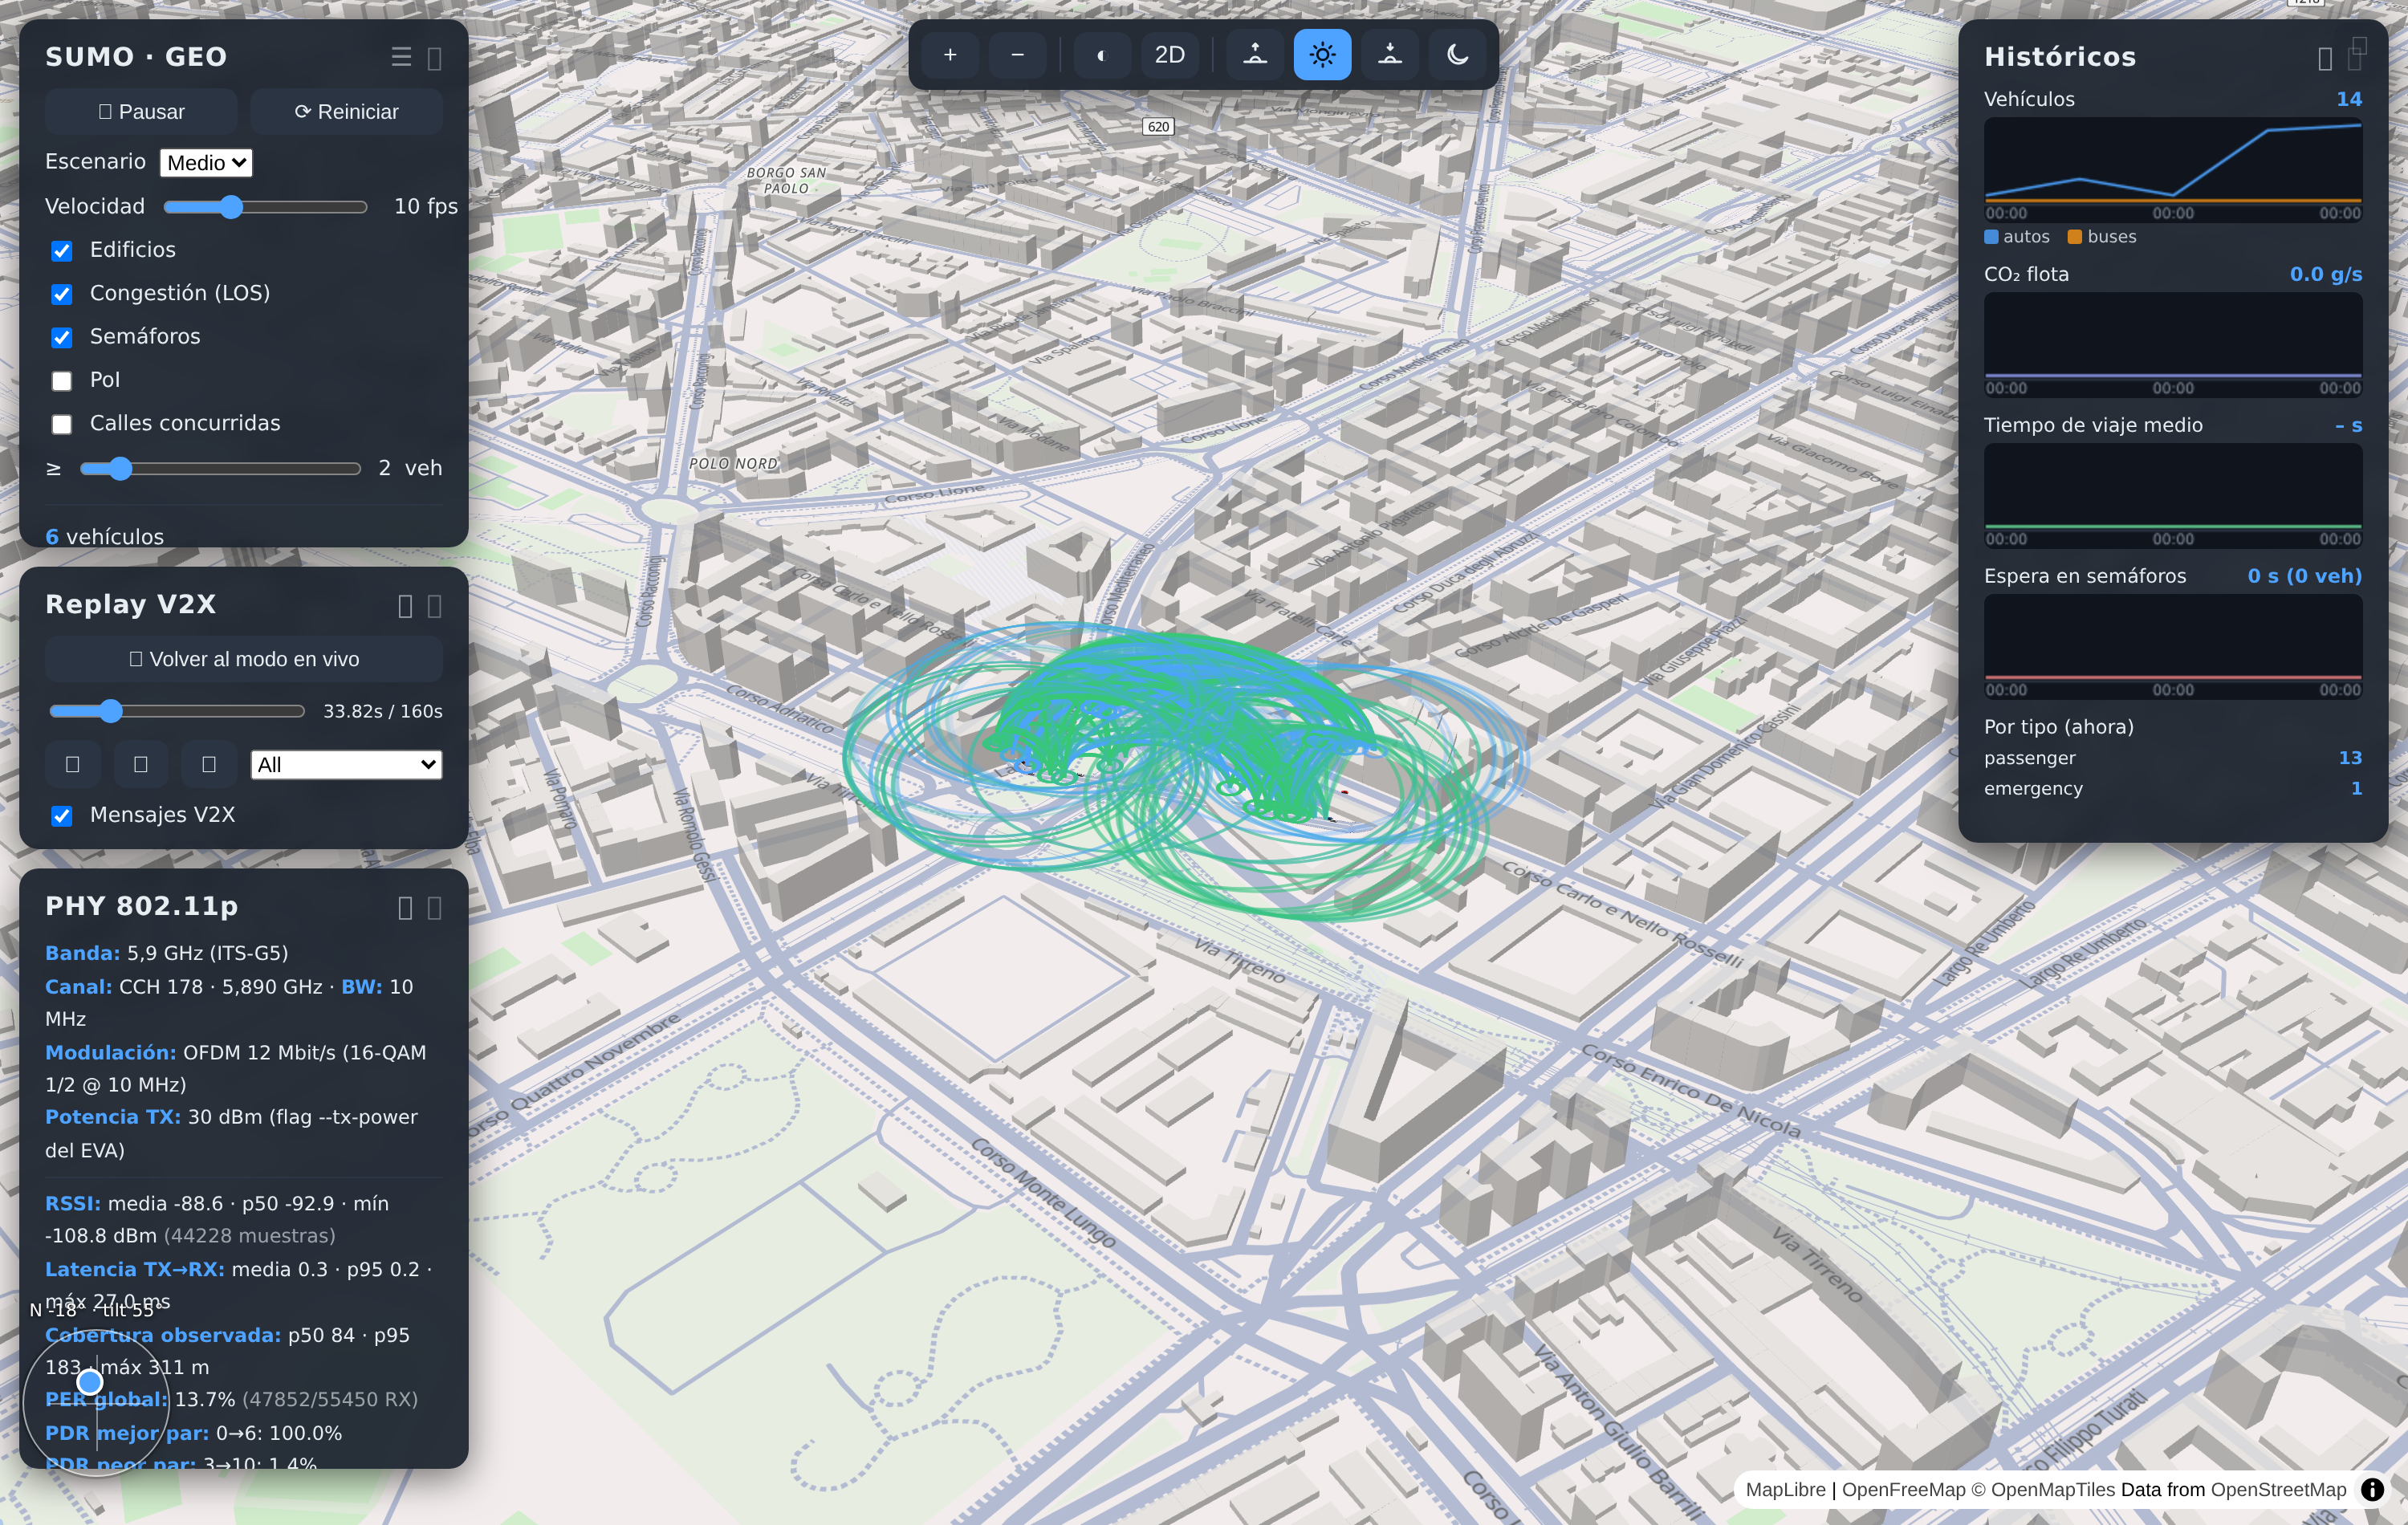
\includegraphics[width=0.94\textwidth]{img/visor_general.png}
\caption{Resultado esperado del nivel 4/5: el visor con la flota del EVA, los
pulsos de transmisión y los paneles de control y métricas.}
\label{fig:final}
\end{figure}

\subsection{Nivel 5 — Replay de mensajes (opcional, cierra el círculo)}

\begin{encontenedor}
\begin{lstlisting}[language=bash]
# tras terminar una corrida del nivel 4:
cp ~/VaN3Twin/ns-3-dev/v2v-EVA-*.pcap ~/results/
\end{lstlisting}
\end{encontenedor}

\begin{ennavegador}
Botón \textbf{Replay pcap} (panel Replay V2X) $\rightarrow$ línea de tiempo,
paso a paso $\blacktriangleleft/\blacktriangleright$ y clic sobre pulsos/arcos
para ver el contenido ASN.1 de cada mensaje. El detalle de este modo es el
tema de la práctica \texttt{Practica\_Replay\_V2X.pdf}.
\end{ennavegador}

% ============================================================================
\section{Problemas frecuentes}
% ============================================================================

\begin{center}
\small
\begin{tabular}{@{}p{0.34\textwidth}p{0.58\textwidth}@{}}
\toprule
\textbf{Síntoma} & \textbf{Causa y solución} \\
\midrule
\texttt{g++: internal compiler error: Killed} durante el build & Falta RAM en Docker: sube a 12--16\,GB (Desktop $\to$ Resources; en WSL2, fichero \texttt{.wslconfig}) y relanza el build \\
\texttt{paths have collided} al clonar & Clonaste el fork de ns-3 en NTFS/APFS: no lo clones — lo gestiona Docker (§\ref{sec:fs}) \\
El build va lentísimo en Windows & Repos clonados en \texttt{/mnt/c}: muévelos al home de WSL2 (\texttt{\textasciitilde{}/}) \\
\texttt{port is already allocated} al \texttt{up} & El visor autónomo (nivel 3) u otra app usa 8000/8081: \texttt{docker compose down} en \texttt{SUMO\_GEO/} \\
\texttt{waiting for 2 clients} eterno & Falta abrir el navegador (nivel 4); o el visor no está arriba: \texttt{docker compose -{}-profile visor up -d} \\
La simulación arranca sin esperar al visor & Faltó \texttt{-{}-num-traci-clients=2} en el comando \\
Visor en negro & \texttt{docker compose logs backend} (desde \texttt{van3twin-docker/}) y \texttt{curl localhost:8000/api/health} \\
\texttt{context not found ../SUMO\_GEO} & Los repos no están uno junto al otro: muévelos o crea el \texttt{.env} con \texttt{SUMO\_GEO\_DIR} \\
\bottomrule
\end{tabular}
\end{center}

% ============================================================================
\section{Entregable}
% ============================================================================

\begin{checkbox}[ final --- capturas a entregar]
\begin{enumerate}[leftmargin=1.6em, itemsep=2pt]
  \item \texttt{docker images} mostrando la imagen \texttt{van3twin}.
  \item Salida del nivel 1 (SUMO) y del nivel 2 (resumen del Metric
        Supervisor).
  \item Navegador en el nivel 3 (Cuenca) y en el nivel 4 (Turín con
        vehículos).
  \item Un mensaje abierto en el nivel 5 (popup con el ASN.1), si llegaste.
\end{enumerate}
\end{checkbox}

\vspace{6pt}\hrule\vspace{6pt}

{\small\emph{Documentos relacionados:}
\texttt{Manual\_Simulacion\_VaN3Twin\_SUMO\_GEO.pdf} (operación diaria del
stack), \texttt{Practica\_Replay\_V2X.pdf} (análisis del intercambio de
mensajes). Repos: \url{https://github.com/Pbarbecho/van3twin-docker},
\url{https://github.com/Pbarbecho/SUMO_GEO},
\url{https://github.com/Pbarbecho/VaN3TwinGEO}.}

\end{document}
